%
% file: internals.tex
%
% author: Chris Cocosco <crisco@bic.mni.mcgill.ca>
%

\documentclass[11pt]{article} 
\usepackage{times}
\usepackage{mathptm}
\usepackage{epsfig}

\topmargin=-0.6in
\textwidth=6.4in
\textheight=9in
\oddsidemargin=0.1in
\evensidemargin=0.1in

\title{JIV Internals}
\author{Chris A.\ Cocosco \\
 \small{$<$\texttt{crisco@bic.mni.mcgill.ca}$>$} }
% FIXME: find a way to automatically include the version number (or
% released date)?
%\date{}

\begin{document}
%\psdraft

\maketitle
\thispagestyle{empty}

\vfill
\newpage

\tableofcontents
\listoffigures
\newpage

\newcommand{\estimate}[2]{[~{\em estimated time required:} {#1}~hrs~{#2}]}


\section{Program Design and Organization}

\subsection{Overview}
\begin{enumerate}
\item The overall design is an object-oriented one. The class
  hierarchy (presented in section~\ref{sec:tree}) attempts to separate
  the common parts of different classes, where possible.
  
  The object interfaces (i.e.\ the inter-class communication) are
  using Java~1.1~AWT's \linebreak \texttt{ImageProducer/ImageObserver}
  and \texttt{EventProducer/EventListener} models.  This makes it easy
  to further expand (and possibly reuse) the software, and to
  interchangeably use \mbox{standard} Java AWT user-interface \&
  image-processing components or custom-written components (AWT is the
  graphical/user-interface part of the standard Java~1.x API).
  
\item Most basic graphical user interface (GUI) building blocks
  (components) are provided by AWT\@.  
  A peculiarity of AWT is that it uses the GUI components provided by
  the underlying platform; while this makes it easier for the user, it
  also makes it harder for the programmer (testing only on one Java
  environment is definitely not enough).

\item Individual volume images are processed and displayed in 8-bit
  indexed-color mode (see figure~\ref{fig:IndividualDataVolumePanel})
  --- in fact, in the JIV input file format the voxel data (intensity
  level) is 8-bit anyway. Moreover, this way the colormap adjustments
  only need to change the palette: it's much faster to change 256
  values rather than $181 \times 217$~!
  
  Combined (blended) volume images are processed and displayed in true
  color mode (see figure~\ref{fig:CombinedDataVolumePanel}) --- color
  blendings/transitions wouldn't look good if reduced to 256 (8-bit)
  colors.

\item Internally, the cursor position is stored as world coordinates
  (float values); this offers more flexibility for future functionality.
  However, inside the slice viewports the visible (cross-hair) cursor
  snaps to the center of the voxels.
  
\item For efficiency reasons, the receivers (listeners) of
  \texttt{PositionEvent}-s are not required to check the range of the
  new position coordinates received.  Thus, it is the responsibility
  of the class generating (sending) such events not to send
  coordinates outside the valid range of the 3D data volume.
  
\item In the image viewports (class \texttt{Slice2DViewport}), AWT
  functions are used for the actual image clipping and scaling (this
  also speeds up the execution, because these functions are generally
  implemented by native code libraries). However, the double-buffering
  of the image viewports had to be explicitly implemented.
  
  Also, a clip window is computed for cross-hair cursor and
  distance-measurement updates. But no clip window is specified for
  slice change, zoom, pan, and viewport resize operations (not a big
  problem, since usually for these operations there isn't much more
  extra screen space, hence the rendering/blit CPU cycles saving won't
  be significant).
  
  The interpolation method used for 2D image scaling is
  nearest-neighbour (provided by AWT). This was chosen mainly for
  interactive speed reasons.
  
\item In the 2D slice viewports, the field of view (FOV), in the
  original image space, is preserved (and centered) when the viewport
  is resized (e.g. when the JIV window is resized). Also, FOV's center
  is maintained when performing zoom-in/out (i.e.\ when changing the
  scale factor).

\item When there are several input volumes with different sampling,
  they are resampled internally to a common sampling during loading (see
  \texttt{VolumeHeader.java} and \texttt{Data3DVolume.java}).

\item The \emph{on-demand} and \emph{hybrid} data download is
  implemented using multiple parallel threads, having a lower
  scheduling priority than the main threads (but not all Java
  runtime environments honor thread priorities...).
  
\item The error handling makes extensive use of Java's elegant
  exception mechanism (\verb+throw+\ and \verb+catch+). Invalid user
  inputs is handled by reverting to the previous (valid) value, or to
  a default value.

\item The code can be divided into two broad groups, based on how it's
  executed:
  \begin{description}
  \item[Initialization:] Code that parses the config file, loads the
    image data, and builds the entire graphical user interface (GUI)
    according to the config file (this includes registering ``event
    listeners'' for all the user-triggered GUI events that we care
    about). After all this is completed, JIV goes to sleep waiting for
    events --- from now on, all the execution will be event-driven.
  \item[Event Handling:] Code that gets called in response to:
    \begin{description}
    \item[user-triggered GUI events:] ``\texttt{InputEvent} listener''
      functions that update the necessary data structures, then issue
      a request to AWT for the screen to be updated.
    \item[AWT-triggered (re)paint requests:] Functions that get called
      by AWT (in response to requests from JIV itself, or from the
      host graphical/windowing system) whenever parts of the screen
      need to be redrawn. 
    \end{description}
  \end{description}



\end{enumerate}


\subsection{Class Hierarchy}
\label{sec:tree}

Classes \& interfaces with names starting with ``\verb+java.+'' are part
of the standard Java~1.1 libraries.  The classes \& interfaces
developed for this project are part of the \verb+jiv+ package: they
have names starting with ``\verb+jiv.+''.

Below, the indentation level corresponds to the inheritance level:
e.g.\ \verb+jiv.LightweightPanel+ is a subclass of
\verb+java.awt.Container+, which in turn is a subclass of
\verb+java.awt.Component+.  Unlike C++, classes in Java can only have
one superclass (can only inherit from one regular class).  However,
Java classes can also inherit from multiple ``interfaces'', which are
classes consisting only of ``abstract methods'', i.e.\ functions
without a specified body (similar to the C++ ``pure virtual
functions'').  In the following, \texttt{implements} means inheriting
from an interface.

%%% Helper commands:
% /data/web/tools/java/Linux/IBMJava2-13/bin/javadoc -package -d javadoc_2/ jiv
% lynx -dump -nolist overview-tree.html > _out
% ...manually cleanup _out ...
%%%%%%%%%%%%%%%%%%%%%%%%%%%%%%%%%%%%%%%%%%%


% this is emacs auto-filled to 90 columns; reduce as needed...

\subsubsection{Interfaces}
\small
\begin{verbatim}
* interface jiv.DataVolumePanel.CoordinateTypes
* interface java.util.EventListener
     + interface jiv.ColormapListener
     + interface jiv.PositionListener
* interface jiv.IndividualDataVolumePanel.ColormapControlMenus
* interface jiv.IndividualDataVolumePanel.ColormapDisplayConstants
* interface jiv.PositionGenerator
\end{verbatim}
\normalsize
   
\subsubsection{Classes}
\small
\begin{verbatim}
* class java.lang.Object
     + class jiv.About
     + class jiv.ColorCoding
     + class
       jiv.CombinedDataVolumePanel.BlendedCombinedImageSource.ByteColormapEntries
     + class
       jiv.CombinedDataVolumePanel.BlendedCombinedImageSource.ShortColormapEntries
     + class jiv.CombinedImageSource (implements
       java.awt.image.ImageProducer, jiv.PositionListener)
          o class
            jiv.CombinedDataVolumePanel.BlendedCombinedImageSource
     + class jiv.CombinedImageSource.InputReader (implements
       java.awt.image.ImageConsumer)
     + class java.awt.Component (implements
       java.awt.image.ImageObserver, java.awt.MenuContainer)
          o class java.awt.Container
               # class jiv.LightweightPanel
                    @ class jiv.CombinedDataVolumePanel.BlendControl
                    @ class jiv.DataVolumePanel.CoordinateFields
                      (implements java.awt.event.ActionListener,
                      jiv.DataVolumePanel.CoordinateTypes,
                      jiv.PositionGenerator, jiv.PositionListener)
                    @ class
                      jiv.IndividualDataVolumePanel.ColormapControl
                      (implements java.awt.event.ActionListener,
                      java.awt.event.AdjustmentListener,
                      jiv.IndividualDataVolumePanel.ColormapControlMenus)
               # class java.awt.Panel
                    @ class java.applet.Applet
                         - class jiv.Main
                    @ class
                      jiv.IndividualDataVolumePanel.ColormapDisplay
                      (implements jiv.ColormapListener,
                      jiv.IndividualDataVolumePanel.ColormapDisplayConstants)
                    @ class jiv.Slice2DViewport (implements
                      jiv.PositionGenerator, jiv.PositionListener)
                         - class jiv.CoronalSlice2DViewport
                         - class jiv.SagittalSlice2DViewport
                         - class jiv.TransverseSlice2DViewport
                    @ class jiv.VerticalLineComponent
               # class java.awt.Window
                    @ class java.awt.Dialog
                         - class jiv.InfoPopupWindow (implements
                           java.awt.event.ActionListener,
                           java.awt.event.WindowListener)
     + class jiv.CoordConv
     + class jiv.Data3DVolume
     + class java.util.EventObject
          o class jiv.ColormapEvent
          o class jiv.PositionEvent
     + class jiv.Help
     + class jiv.Main.PanelStruct
     + class jiv.Main.VolumeStruct
     + class java.awt.image.MemoryImageSource (implements
       java.awt.image.ImageProducer)
          o class jiv.SliceImageProducer (implements
            jiv.ColormapListener, jiv.PositionListener)
               # class jiv.CoronalSliceImageProducer
               # class jiv.SagittalSliceImageProducer
               # class jiv.TransverseSliceImageProducer
     + class java.awt.MenuComponent
          o class java.awt.MenuItem
               # class java.awt.CheckboxMenuItem
                    @ class jiv.PositionSyncMenuItem
               # class java.awt.Menu (implements java.awt.MenuContainer)
                    @ class jiv.ChoiceMenu
               # class jiv.QuitMenuItem
     + class jiv.MultiLineStringBuffer
     + class jiv.Point3Dfloat
     + class jiv.Point3Dint
     + class jiv.PositionListenerAdapter (implements
       jiv.PositionListener)
          o class jiv.DataVolumePanel (implements
            jiv.PositionGenerator)
               # class jiv.CombinedDataVolumePanel
               # class jiv.IndividualDataVolumePanel
          o class jiv.PositionGateway (implements
            jiv.PositionGenerator)
     + class java.awt.geom.RectangularShape (implements
       java.lang.Cloneable, java.awt.Shape)
          o class java.awt.geom.Rectangle2D
               # class java.awt.Rectangle (implements
                 java.awt.Shape)
                    @ class jiv.Rectangle2
     + class jiv.StandaloneAppletContext (implements
       java.applet.AppletContext)
     + class jiv.StandaloneAppletStub (implements
       java.applet.AppletStub)
     + class jiv.Util
     + class jiv.ViewportCursor
     + class jiv.ViewportDistanceDisplay
     + class jiv.VolumeHeader
     + class jiv.VolumeHeader.ResampleTable
\end{verbatim}
\normalsize
 %Ok

\subsection{Class Summary}
\label{sec:summary}

\newcommand{\entityintro}[3]{ \item[{#1}] ~\\ {#3} }
\newenvironment{entityenvironment}{\begin{description}}{\end{description}}

%%%%%%
% Helper command:
%
% ls -1 jiv > _sorted_java_files
% /data/web/tools/java/Linux/IBMJava2-13/bin/javadoc -output texdoclet/doc.tex -doclet com.c2_tech.doclets.TexDoclet -docletpath /data/nil/crisco/lib/java/texdoclet.jar -noinherited -package @_sorted_java_files
% 
%%%%%%%%%%%%%%%%%%%%%%%%%%%



%\newcommand{\entityintro}[3]{ \subparagraph{{#1}} {#3} }

% \newcommand{\entityintro}[3]{%
%   \hbox to \hsize{%
%     \vbox{%
%       \hbox to .2in{}%
%     }%
%     {\bf #1}%
%   }
%   \makebox[\hsize]{%
%     \parbox{.4in}{}%
%     \parbox[l]{5in}{%
%       \vspace{1mm}\it%
%       #3%
%       \vspace{1mm}%
%     }%
%   }%
% }

\subsubsection{Interfaces}
\begin{entityenvironment}
\entityintro{ColormapListener}{l0}{The interface that all {\tt ColormapEvent} listener
 (receiver) classes must implement.}
\entityintro{DataVolumePanel.CoordinateTypes}{l1}{Support interface for the inner class
 {\tt DataVolumePanel.CoordinateFields}.}
\entityintro{IndividualDataVolumePanel.ColormapControlMenus}{l2}{Support interface for the inner class
 {\tt IndividualDataVolumePanel.ColormapControl}.}
\entityintro{IndividualDataVolumePanel.ColormapDisplayConstants}{l3}{Support interface for the inner class
 {\tt IndividualDataVolumePanel.ColormapDisplay}.}
\entityintro{PositionGenerator}{l4}{The interface that all classes sending {\tt PositionEvent}-s
 must implement.}
\entityintro{PositionListener}{l5}{The interface that all {\tt PositionEvent} listener
 (receiver) classes must implement.}
\end{entityenvironment}
   
\subsubsection{Classes}
\begin{entityenvironment}
\entityintro{About}{l6}{Static class providing text descriptions (including copyright 
 and license) for this software.}
\entityintro{ChoiceMenu}{l7}{A choice menu that allows to select one item from it, radio-buttons
 style.}
\entityintro{ColorCoding}{l8}{Produces 8bit colormaps (palettes), according to given
 specifications.}
\entityintro{ColormapEvent}{l9}{An event type used for communicating colormap changes.}
\entityintro{CombinedDataVolumePanel}{l10}{Implements the volume panel functionality specific to panels
 displaying a combination of two image volumes.}
\entityintro{CombinedDataVolumePanel.BlendedCombinedImageSource}{l11}{Member (inner) class: a {\tt CombinedImageSource} that
 uses an adjustable blending factor for combining two images
 (in RGB color space).}
\entityintro{CombinedDataVolumePanel.BlendedCombinedImageSource.ByteColormapEntries}{l12}{helper class (a member$/$inner class)}
\entityintro{CombinedDataVolumePanel.BlendedCombinedImageSource.ShortColormapEntries}{l13}{helper class (a member$/$inner class)}
\entityintro{CombinedDataVolumePanel.BlendControl}{l14}{Member (inner) class: the user interface input controls for
 adjusting the blending factor.}
\entityintro{CombinedImageSource}{l15}{Template for a class that combines two source images into one
 output image using the
 {\tt ImageProducer}$/${\tt ImageConsumer}
 interfaces.}
\entityintro{CombinedImageSource.InputReader}{l16}{Inner (member) class: the interface to the source
 {\tt ImageProducer}-s.}
\entityintro{CoordConv}{l17}{Functions for converting 3D positions between the "voxel" (array
 index) and "world" coordinate systems.}
\entityintro{CoronalSlice2DViewport}{l18}{A {\tt Slice2DViewport} customized for "coronal"
 (Y=constant) slices.}
\entityintro{CoronalSliceImageProducer}{l19}{A {\tt SliceImageProducer} customized for "coronal"
 (Y=constant) 2D slices.}
\entityintro{Data3DVolume}{l20}{Loads, stores, and provides access to a 3D image volume.}
\entityintro{DataVolumePanel}{l21}{Provides the functionality common for both volume panel types
 (individual and combined).}
\entityintro{DataVolumePanel.CoordinateFields}{l22}{Member (inner) class: the textual coordinate display$/$input
 boxes ("fields").}
\entityintro{Help}{l23}{Static class providing the help text functionality.}
\entityintro{IndividualDataVolumePanel}{l24}{Provides the volume panel functionality specific to panels
 displaying a single image volume.}
\entityintro{IndividualDataVolumePanel.ColormapControl}{l25}{Member (inner) class : the user interface input
 controls for adjusting the colormap.}
\entityintro{IndividualDataVolumePanel.ColormapDisplay}{l26}{Member (inner) class: produces a visual representation of
 the current colormap.}
\entityintro{InfoPopupWindow}{l27}{An information popup window, complete with an Ok button to dismiss it.}
\entityintro{LightweightPanel}{l28}{A "lightweight" alternative to {\tt java.awt.Panel}; it
 doesn't have a native peer, hence should use fewer system
 resources.}
\entityintro{Main}{l29}{The entry-point class, both when running as an applet and when
 running as a standalone application.}
\entityintro{Main.VolumeStruct}{l30}{Helper data structure: represents an individual 3D image
 volume.}
\entityintro{Main.PanelStruct}{l31}{Helper data structure: represents a GUI panel.}
\entityintro{MultiLineStringBuffer}{l32}{A buffer for multi-line text.}
\entityintro{Point3Dfloat}{l33}{A tuple of (x,y,z) floating point coordinates.}
\entityintro{Point3Dint}{l34}{A tuple of (x,y,z) integer coordinates.}
\entityintro{PositionEvent}{l35}{An event type used for communicating position (cursor) changes, as
 "world" coordinates.}
\entityintro{PositionGateway}{l36}{Provides a gateway ("firewall") for exchanging
 {\tt PositionEvent}-s between two sets of
 {\tt PositionListener$/$PositionGenerator}-s.}
\entityintro{PositionListenerAdapter}{l37}{An adapter (convenience) class for receiving
 {\tt PositionEvent}-s.}
\entityintro{PositionSyncMenuItem}{l38}{A menu item that toggles the cursor position sync mode.}
\entityintro{QuitMenuItem}{l39}{An application 'quit' menu item.}
\entityintro{Rectangle2}{l40}{An enhancement of the stock AWT {\tt java.awt.Rectangle}.}
\entityintro{SagittalSlice2DViewport}{l41}{A {\tt Slice2DViewport} customized for "sagittal"
 (X=constant) slices.}
\entityintro{SagittalSliceImageProducer}{l42}{A {\tt SliceImageProducer} customized for "sagittal"
 (X=constant) 2D slices.}
\entityintro{Slice2DViewport}{l43}{Provides the orientation-independent functionality of displaying 2D
 slice image data in a viewport, and of allowing the user to
 interact with it.}
\entityintro{SliceImageProducer}{l44}{An {\tt ImageProducer} that provides the
 orientation-independent functionality of producing 2D slice image
 data.}
\entityintro{StandaloneAppletContext}{l45}{Provides a (very basic) {\tt AppletContext}, allowing an
 applet to be run as a standalone application, without an
 appletviewer or web browser.}
\entityintro{StandaloneAppletStub}{l46}{Provides a (very basic) {\tt AppletStub}, allowing an
 applet to be run as a standalone application, without an
 appletviewer or web browser.}
\entityintro{TransverseSlice2DViewport}{l47}{A {\tt Slice2DViewport} customized for "transverse"
 (Z=constant) slices.}
\entityintro{TransverseSliceImageProducer}{l48}{A {\tt SliceImageProducer} customized for "transverse"
 (Z=constant) 2D slices.}
\entityintro{Util}{l49}{A collection of various ({\tt static}) utility functions.}
\entityintro{VerticalLineComponent}{l50}{A stretchable vertical line (useful as a separator).}
\entityintro{ViewportCursor}{l51}{A graphical position cursor.}
\entityintro{ViewportDistanceDisplay}{l52}{Graphically displays a "distance measurement" rubber band, complete
 with a supplied text.}
\entityintro{VolumeHeader}{l53}{Loads, stores, and provides access to the header info of a 
 3D image volume.}
\entityintro{VolumeHeader.ResampleTable}{l54}{...no description...}
\end{entityenvironment}

 %Ok

%%%%%% TODO: state diagram for interactions inside Slice2DVport !!??

\begin{figure}[p]
\begin{center}
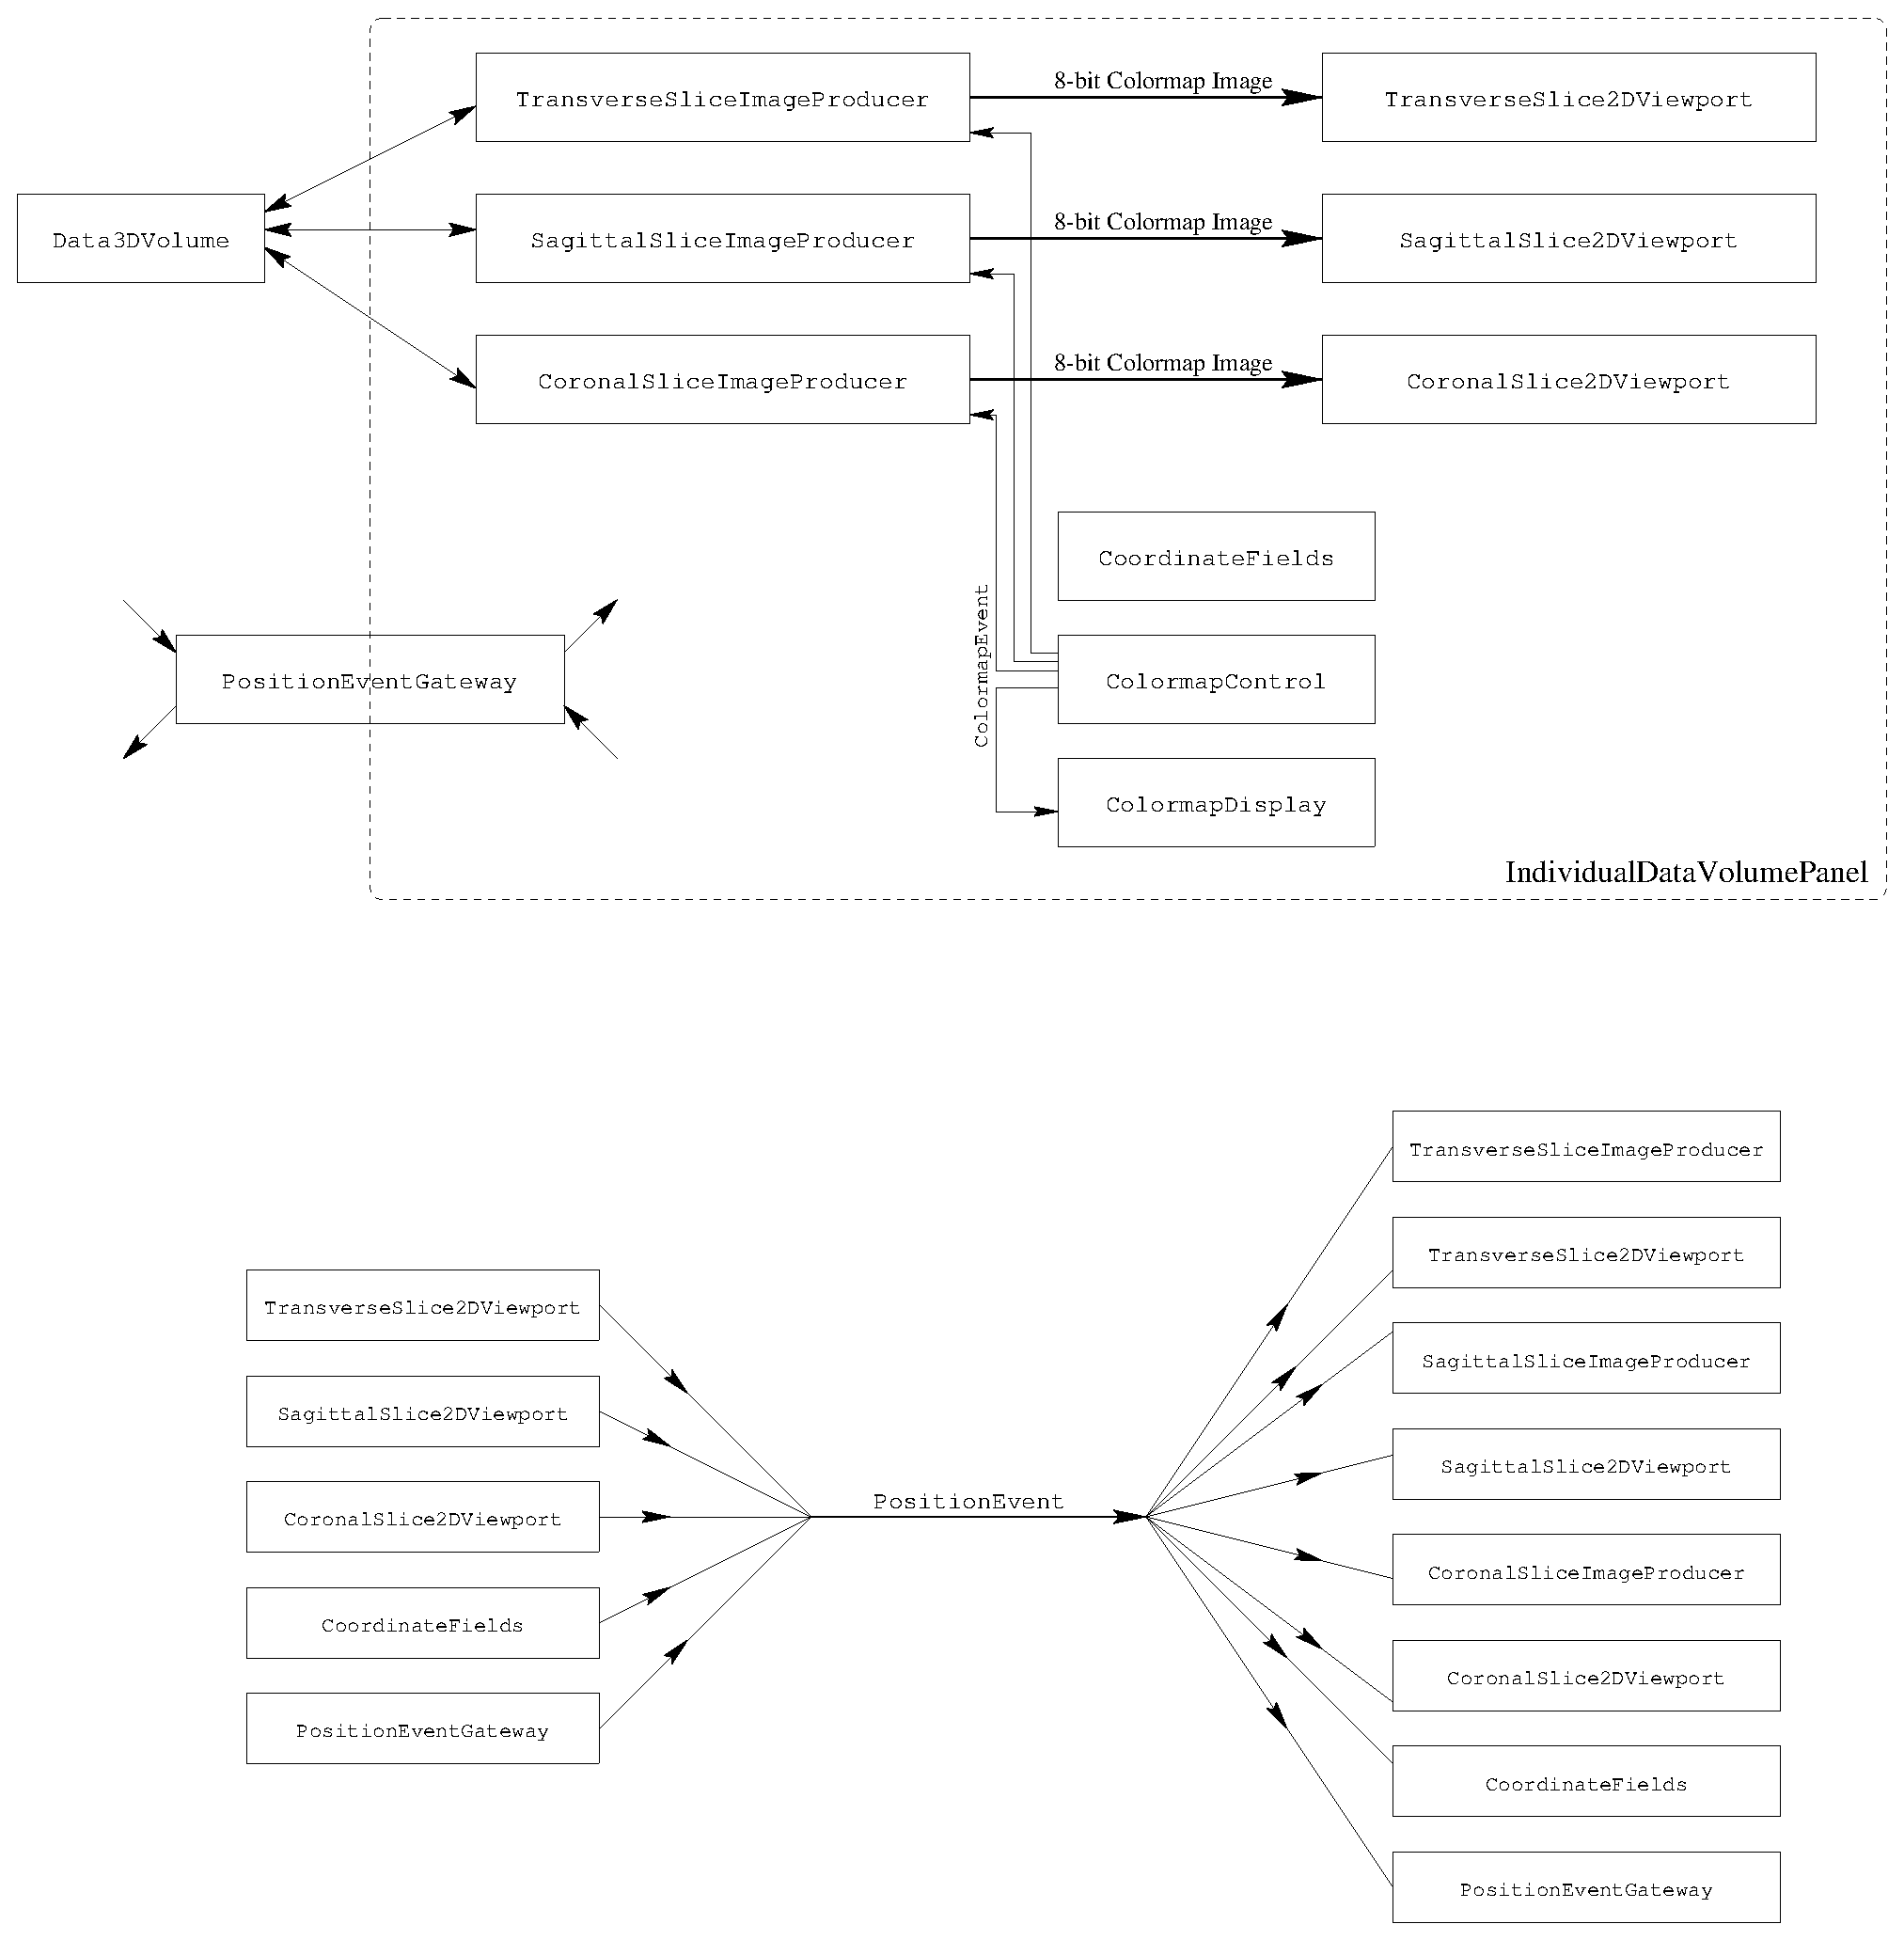
\epsfig{file=figs/IndividualDataVolumePanel.eps,width=\linewidth}
\end{center}
\caption[Overview of interactions in
\texttt{IndividualDataVolumePanel}]{Overview of interactions in
  \texttt{IndividualDataVolumePanel}. For clarity, the
  \mbox{\texttt{PositionEvent}} flow is shown separately in the bottom
  figure. The \mbox{\texttt{PositionEventGateway}} is used for sharing
  cursor position information with the other volume panels when the
  \mbox{\emph{Sync all cursors}} mode is active.}
\label{fig:IndividualDataVolumePanel}
\end{figure}

\begin{figure}[p]
\begin{center}
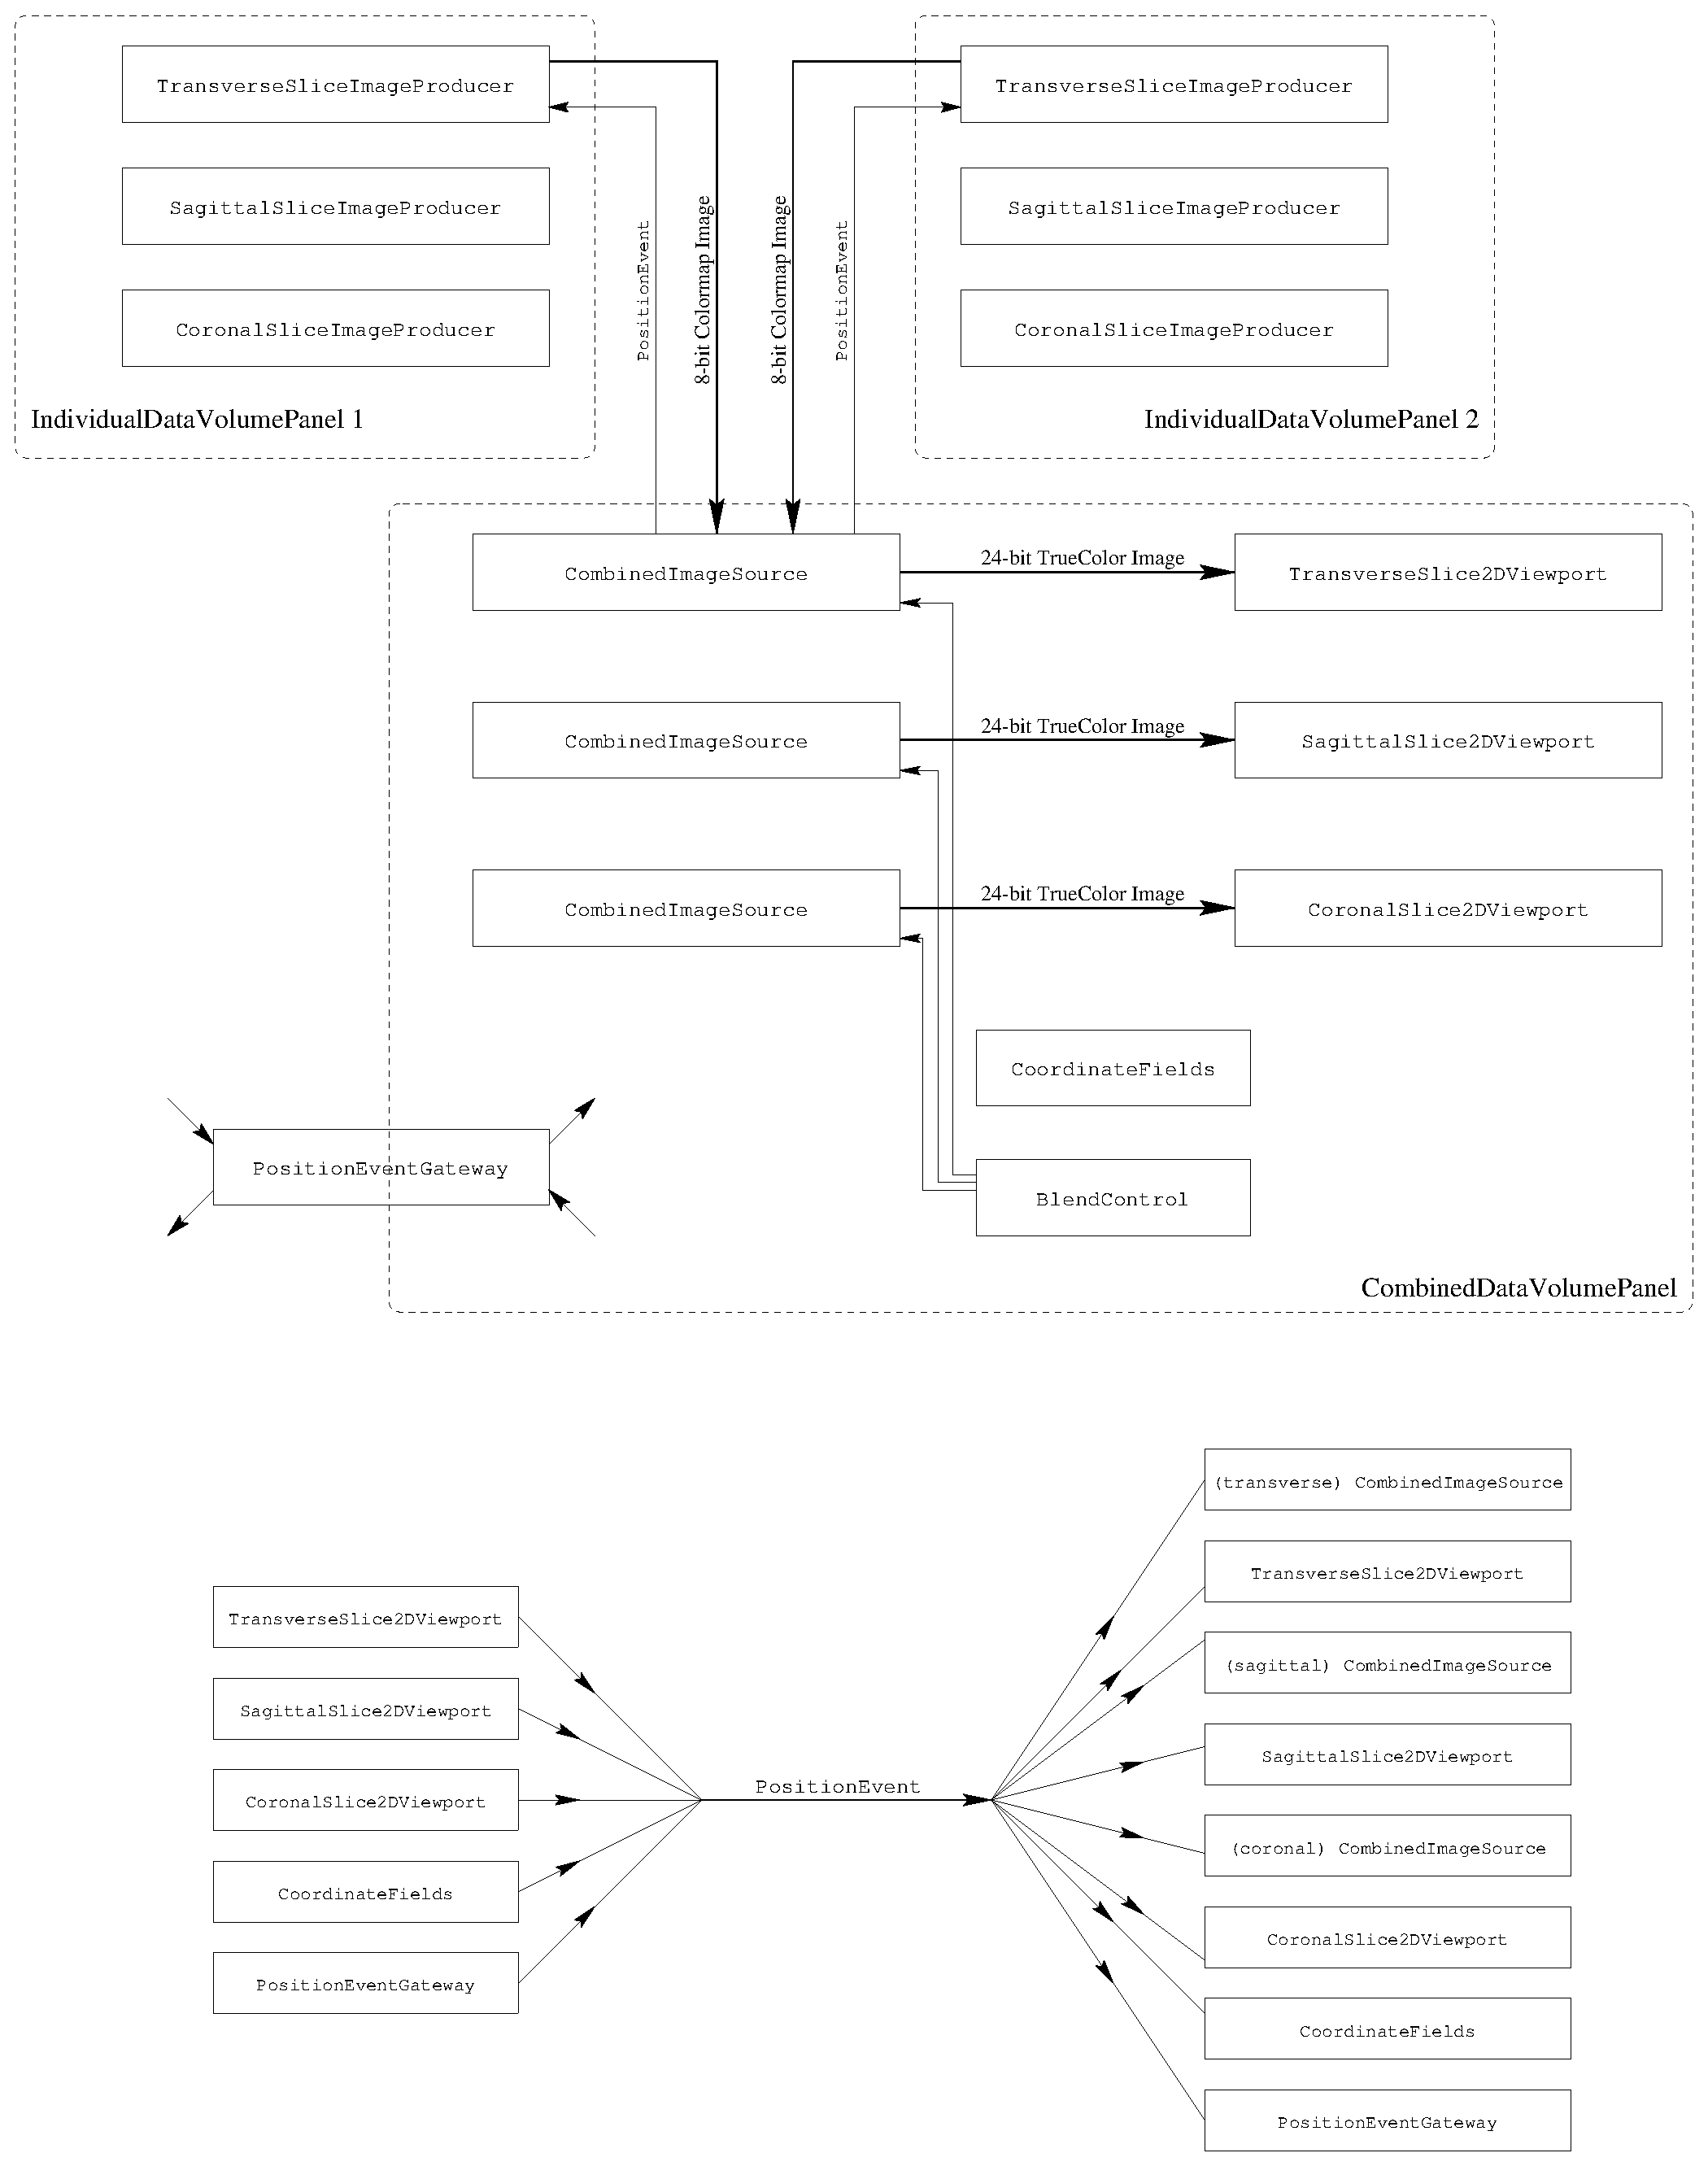
\epsfig{file=figs/CombinedDataVolumePanel.eps,width=\linewidth}
\end{center}
\caption[Overview of interactions in
\texttt{CombinedDataVolumePanel}]{Overview of interactions in
  \texttt{CombinedDataVolumePanel}.  For clarity, the
  \mbox{\texttt{PositionEvent}} flow is shown separately in the bottom
  figure.}
\label{fig:CombinedDataVolumePanel}
\end{figure}


\subsection{Implementation: Problems Encountered}
\label{sec:problems-encountered}

\begin{itemize}
\item Since existing (no-cost) Java compilers do a very poor job at
  optimizing the byte-code, time was spent on hand-optimizing the
  time-consuming bits of the code (needed in order to obtain good
  interactive response of the viewer).
\item In Java there's no way of allocating non-primitive data types
  (objects) on the stack (for local/temporary variables); only a
  reference (pointer) to objects can go on the stack. Moreover, the
  heap memory manager (which uses a garbage-collection model) of
  Java~1.1 runtime environments seems not to be very efficient in
  terms of overhead time and memory usage. Thus, in order to improve
  the response time, and also minimize the memory footprint increase
  during execution, most local object variables that are frequently
  used were manually pre-allocated and reused after that; such
  variables are named \verb+__methodname_variablename+.
\item The development environment used (IBM JDK for Linux,
  version~1.1.8 -- a port of Sun's JDK~1.1.8) has several serious bugs
  in the compiler.  Workarounds had to be found \ldots Also, there's
  also a significant memory leak in one standard AWT class: 
  \verb+java.awt.image.ReplicateScaleFilter+.
%   more: x-platform portability (Win32: popups, auto-repeating
%   keys, MouseEvent bugs, scrollbars returning vals out of range,
%   \ldots)
  
\item The file \verb+jiv/JAVA_NOTES+ (in the source code directory)
  contains more notes about undocumented/obscure issues with the Java
  language and the version 1.1 JDK (Java Development Kit) \ldots

\end{itemize}


\end{document}

